% Goes in previous section: In lattice QCD, we represent quark fields directly as Grassmann-valued fields on spacetime lattice sites, but we represent gluon fields as discretized gauge-transporters called \textit{link variables}, which are envisaged as directional links between lattice sites. (Gatt. and Lang pg. 34-35)
\section{Basic Building Blocks}
    Quarks and gluons are the principle objects of quantum chromodynamics, and form the hadrons which we wish to study. Hence, the operators we use to create hadrons on the lattice are constructed using building blocks of quark and gluon fields. Since hadrons are not point-like objects, but extended composite objects, we form our hadron operators out of \textit{covariantly-displaced} quark fields. In calculating correlator observables on the lattice, two important obstacles must be confronted:  noise, and excited-state contamination. With these challenges in mind, our basic building blocks include so-called \textit{stout-smeared} gauge-link field variables and \textit{LapH-smeared} quark field variables. We will see that the stout smearing procedure leads dramatically reduced noise in the evaluation of correlators constructed with displaced operators, and that the LapH-smearing procedure drastically attenuates contributions from higher-lying modes of the theory. Both of these procedures are crucial for extracting the energy spectrum, as we will see in Chapter~\ref{ch:analysis}.
    \subsection{Stout Smearing}
    Ref.~\cite{PhysRevD.69.054501} describes a smearing procedure for link variables known as stout smearing, which is outlined here. Define $C_\mu(x)$ as the following weighted sum of perpendicular link-variable staples (depicted in Fig.~\ref{fig:staples}) beginning at a lattice site $x$ and terminating at a neighboring site $x + \hat\mu$,
    \begin{equation}
        C_{\mu}(x)= \sum_{\nu \neq \mu} \rho_{\mu \nu}\left(U_{\nu}(x) U_{\mu}(x+\hat{\nu}) U_{\nu}^{\dagger}(x+\hat{\mu})\right.\left.+U_{\nu}^{\dagger}(x-\hat{\nu}) U_{\mu}(x-\hat{\nu}) U_{\nu}(x-\hat{\nu}+\hat{\mu})\right),
    \end{equation}
    where $\rho_{\mu\nu}$ are tunable real parameters, and $\hat\mu$ and $\hat\nu$ are unit vectors on the lattice. We use the following weights, which amount to smearing spacial link variables only,
    \begin{equation}
        \rho_{j k}=\rho, \quad \rho_{4 \mu}=\rho_{\mu 4}=0.
    \end{equation}
    % To do: make note of positive definiteness, add bits about parameters we use.
    Next, define a matrix $Q_\mu(x)$ in SU($N$) by
    \begin{equation}
        \begin{aligned}
            Q_{\mu}(x)&=\frac{i}{2}\left(\Omega_{\mu}^{\dagger}(x)-\Omega_{\mu}(x)\right)-\frac{i}{2 N} \operatorname{Tr}\left(\Omega_{\mu}^{\dagger}(x)-\Omega_{\mu}(x)\right) \\
            \Omega_{\mu}(x)&=C_{\mu}(x) U_{\mu}^{\dagger}(x), \quad \text { (no summation over } \mu).
        \end{aligned}
    \end{equation}
    Being both Hermitian and traceless, $Q_\mu(x)$ is also in the Lie algebra $\mathfrak{su}(2)$, and therefore $e^{Q\mu(x)} \in \mathrm{SU}(N)$. Then define an iterative process whereby a link variable at step $n + 1$ is related to a link variable at step $n$ as,
    \begin{equation}
        U_{\mu}^{(n+1)}(x)=\exp \left(i Q_{\mu}^{(n)}(x)\right) U_{\mu}^{(n)}(x).
    \end{equation}
    Since the link variables we start with are in SU($N$) and so is $e^{Q\mu(x)}$, we guarantee that each link variable in this iteration is also in SU($N$). This ensures that transforming the link variables in this way preserves the property that they are members of the SU(3) gauge group.

    This smearing procedure can be iterated $n_\rho$ times to produce what we refer to as \textit{stout links} and denote by $\tilde{U}_\mu(x)$:
    \begin{equation}
        U \rightarrow U^{(1)} \rightarrow U^{(2)} \rightarrow \cdots \rightarrow U^{\left(n_{\rho}\right)} \equiv \tilde{U}.
    \end{equation}
    There are two important takeaways of this procedure: only the spatial links are smeared, and all of the symmetries of the original links are preserved.
    
    \subsection{LapH Smearing}
    Recall that one can approximate the second derivative of a single-variable function $f$ at a point $x$ as, $f^{\prime\prime}(x) \approx \frac{f(x+a) + f(x-a) - 2f(x)}{2a}$, for small $a$. Hence, taking a second derivative provides one convention for smearing a function, as it performs a weighted average of the function in the neighborhood of a point $x$. On the lattice, we look to the three-dimensional gauge-covariant Laplacian (GCL) to accomplish quark field smearing in a way that preserves the gauge symmetries of the action. In terms of stout smeared link variables, $\tilde U_j(x)$, the gauge-covariant Laplacian is defined as,
    \begin{equation}\label{eq:quark_smearing}
    \begin{aligned} \tilde{\Delta} O(x) &=\sum_{k=1}^{3}\left(\tilde{U}_{k}(x) O(x+\hat{k})+\tilde{U}_{k}^{\dagger}(x-\hat{k}) O(x-\hat{k})-2 O(x)\right), \\ \overline{O}(x) \overleftarrow{\Delta} &=\sum_{k=1}^{3}\left(\overline{O}(x+\hat{k}) \tilde{U}_{k}^{\dagger}(x)+\overline{O}(x-\hat{k}) \tilde{U}_{k}(x-\hat{k})-2 \overline{O}(x)\right). \end{aligned}
    \end{equation}
    Acting the GCL on any operator $O(x)$ preserves all of the single-time-slice symmetry properties of that operator, and therefore so does acting it on that operator any number of times~\cite{cite:spectroscopy}. It can be shown~\cite{ref:spectroscopy} that when we act the GCL on our quark fields, $\psi$ and $\overline\psi$, which are Grassmann-valued, the resultant smeared fields, $\widetilde{\psi}$ and $\widetilde{\overline\psi}$, are also Grassmann-valued. One scheme for quark field smearing, defined by~\cite{24spectroscopy}, is,
    \begin{equation}
    \begin{aligned} \widetilde{\psi}(x) &=\left(1+\frac{\sigma_{s}^{2}}{4 n_{\sigma}} \widetilde{\Delta}\right)^{n_{\sigma}} \psi(x), \\ \widetilde{\overline\chi}(x) &=\overline{\chi}(x)\left(1+\frac{\sigma_{s}^{2}}{4 n_{\sigma}} \overleftarrow{\Delta}\right)^{n_{\sigma}}, \end{aligned}
    \end{equation}
    where $\sigma_s\in\mathbb{R}$ and $n_\sigma\in\mathbb{Z}$ are tunable parameters.

    We can now examine the effect of both link smearing and quark field smearing, using the procedures presented thus far. Fig.~\ref{fig:meff-smearing} demonstrates how quark field smearing drastically reduces excited-state contamination in the correlator calculations, and how link smearing drastically reduces signal noise.
    \begin{figure}
        \centering
        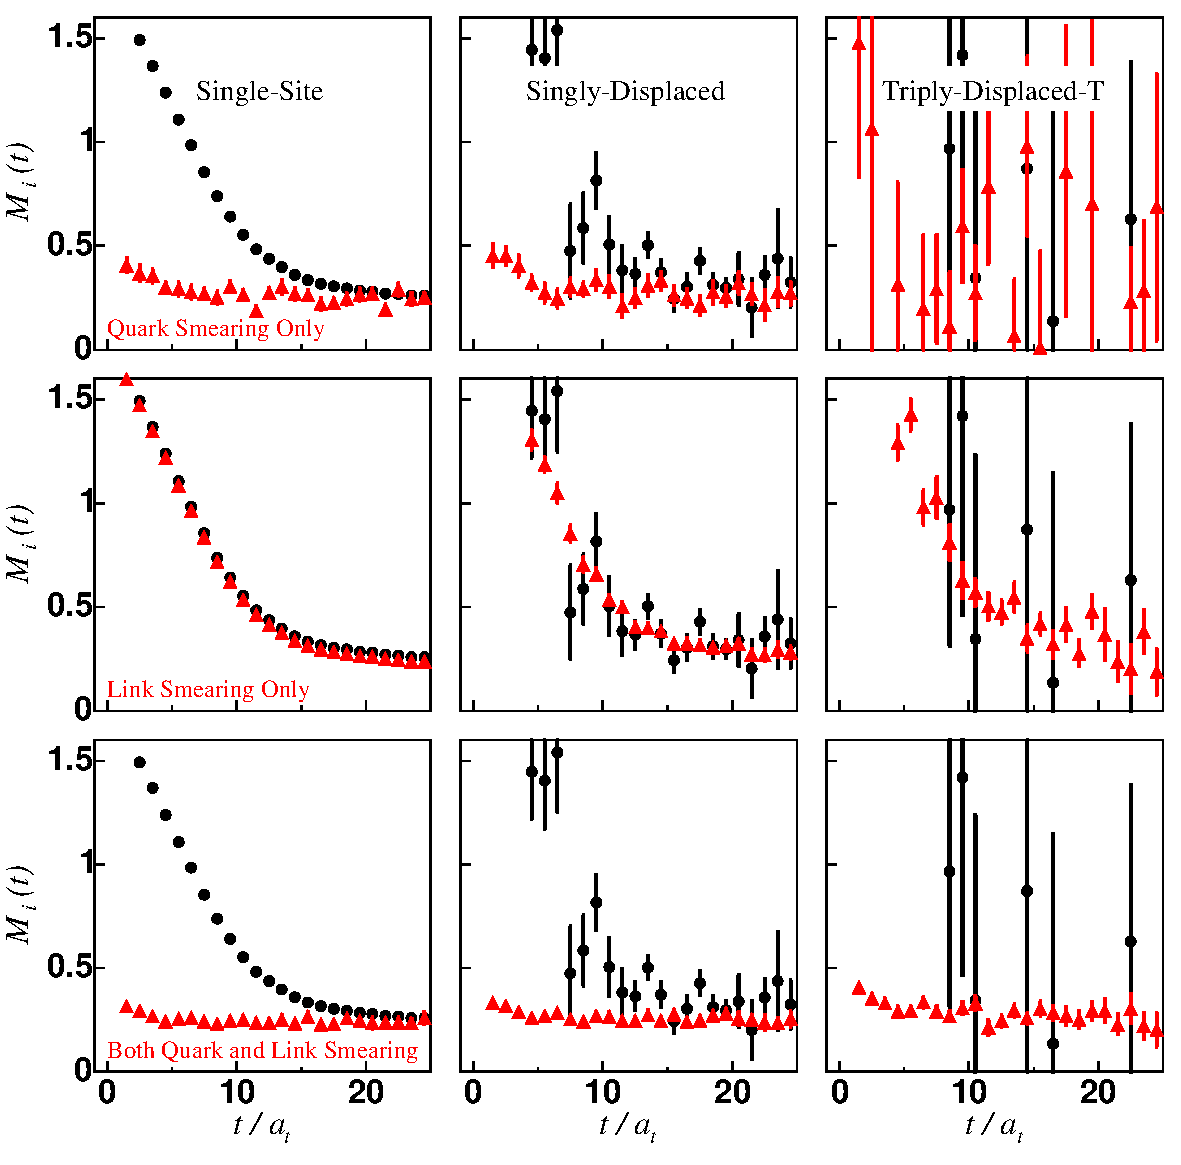
\includegraphics[scale=0.8]{figures/meff-smearing.pdf}
        \caption{Insert caption, cite spectroscopy.}\label{fig:meff-smearing}
    \end{figure}
    
    $\tilde\Delta$ is Hermitian, and we define its eigenvalues as $-\lambda^{(k)}$ (ordered by increasing $\lambda^{(k)}$) and their corresponding orthonormal eigenvectors as $v^{(k)}$. Then, if we define the smearing kernel in Eq.~\ref{eq:quark_smearing} as $K=\left(1+\frac{\sigma_{s}^{2}}{4 n_{\sigma}} \widetilde{\Delta}\right)^{n_{\sigma}}$, we can express the kernel in the eigenbasis of the GCL:
    \begin{equation}
        K_{a b}(x, y)=\delta_{x_{4}, y_{4}} \sum_{k} w_{k}\,v_{a}^{(k)}(x) v_{b}^{(k)}(y)^{*},
    \end{equation}
    where we suppress the flavor index, and where $w_k\in\mathbb{R}^+$. Since $K$ is written in terms of $\tilde\Delta$, it is trivial to write down,
    \begin{equation}
        w_{k}=\left(1-\frac{\sigma_{s}^{2}}{4 n_{\sigma}} \lambda^{(k)}\right)^{n_{\sigma}}.
    \end{equation}
    It is then also easy to see that,
    \begin{equation}
        \lim _{n_{\sigma} \rightarrow \infty} w_{k}=\exp \left(-\frac{1}{4} \sigma_{s}^{2} \lambda^{(k)}\right).
    \end{equation}
    We can now see the advantage of working in the eigenbasis of the GCL: the weights, $w_{k}$, of higher modes of $\tilde\Delta$ are exponentially suppressed. We can then investigate the possibility of modifying the weights to neglect higher-lying contributions. One simple way to accomplish this is the so-called \emph{Laplacian Heaviside} (LapH) smearing scheme, introduced by Peardon, Morningstar, et al. in ~\cite{PhysRevD.80.054506}. This procedure sets the weights to be,
    \begin{equation}
        w_{k}=\Theta\left(\sigma_{s}^{2}-\lambda^{(k)}\right),
    \end{equation}
    where $\Theta$ is the Heaviside step function, and $\sigma_s^2$ acts as a hard cutoff. The LapH smearing kernel is now defined as
    \begin{equation}
        \mathcal{S}=\Theta\left(\sigma_{s}^{2}+\widetilde{\Delta}\right),
    \end{equation}
    and our smeared quark fields are now given by
    \begin{equation}
        \widetilde\psi(x) = \mathcal{S}\psi(x).
    \end{equation}

    \subsection{Displacements}
    The motivation for displacing the quark fields is hadrons are objects which are extended in space. Therefore, if we hope to capture radial and orbital structure when computing the hadronic correlation functions, then we must displace the quark fields, and do so in a gauge-covariant way. The displacements we consider are straight-path displacements along the spatial lattice unit vectors: $j = \pm 1, \pm 2, \pm 3$. We define the gauge-covariant displacement operator in the $j^{\mathrm{th}}$ direction by,
    \begin{equation}
        \widetilde{D}_{j}^{(p)}\left(x, x^{\prime}\right)=\widetilde{U}_{j}(x) \widetilde{U}_{j}(x+\hat{j}) \ldots \widetilde{U}_{j}(x+(p-1) \hat{j}) \delta_{x^{\prime}, x+p \hat{j}},
    \end{equation}
    where $p \geq 1$ denotes the number of steps in by which the field is displaced. For convenience, we also define a zero-displacement operator, $\widetilde{D}_{0}^{(p)}\left(x, x^{\prime}\right)=\delta_{x x^{\prime}}.$ Including color indices $a$ and $a^\prime$, it can be shown that $\widetilde{D}_{j}^{(p) \dagger}\left(x, x^{\prime}\right)^{a a^{\prime}}=\widetilde{D}_{-j}^{(p)}\left(x, x^{\prime}\right)^{a a^{\prime}}.$ From this, the following useful properties can be derived:
    \begin{equation}
        \begin{aligned}
            \left(\widetilde{D}_{j}^{(p)} \psi\right)(x)&=\sum_{x^{\prime}} \widetilde{D}_{j}^{(p)}\left(x, x^{\prime}\right) \psi\left(x^{\prime}\right)=\widetilde{U}_{j}(x) \widetilde{U}_{j}(x+\hat{j}) \ldots \widetilde{U}_{j}(x+(p-1) \hat{j}) \psi(x+p \hat{j}),\\
            \left(\overline{\chi} \widetilde{D}_{j}^{(p) \dagger}\right)(x)&=\sum_{x^{\prime}} \overline{\chi}\left(x^{\prime}\right) \widetilde{D}_{j}^{(p) \dagger}\left(x^{\prime}, x\right)=\sum_{x^{\prime}} \overline{\chi}\left(x^{\prime}\right) \widetilde{D}_{-j}^{(p)}\left(x^{\prime}, x\right)\\
            &=\overline{\chi}(x+p \hat{j}) \widetilde{U}_{j}^{\dagger}(x+(p-1) \hat{j}) \ldots \widetilde{U}_{j}^{\dagger}(x+\hat{j}) \widetilde{U}_{j}^{\dagger}(x),
        \end{aligned}
    \end{equation}
    from which it can be seen,
    \begin{equation}
        \overline{\chi}(x)\left(\widetilde{D}_{j}^{(p)} \psi\right)(x)=\left(\overline{\chi} \widetilde{D}_{j}^{(p)}\right)(x) \psi(x).
    \end{equation}
    {\color{red}Why do we have to show associativity? Why would it not be obvious?}

    The final building blocks for our hadronic operators are \emph{covariantly-displaced, smeared quark fields} and can be summarized as follows:
    \begin{equation}
        \boxed{\left(\widetilde{D}_{j_{1}}^{(p)} \ldots \widetilde{D}_{j_{n}}^{(p)} \widetilde{\psi}\right)_{a \alpha}^{A}, \quad\left(\widetilde{\chi} \widetilde{D}_{j_{1}}^{(p) \dagger} \ldots \widetilde{D}_{j_{n}}^{(p) \dagger}\right)_{a \alpha}^{A}, \quad-3 \leq j_{i} \leq 3.}
    \end{equation}
    {\color{red}Add in graphics showing types of displacements we use.}

    \section{Symmetries on the Lattice}
    Symmetries are very useful for characterizing and labeling stationary states in quantum mechanics. Conserved quantities, such as momentum and charge, emerge from the symmetries of a given system, and so in order to identify the relevant quantum numbers of a theory, we must identify its relevant symmetries. The primary symmetries we are interested in are: (cubic) rotations, $G$-parity, isospin, and flavor. SU(3) gauge symmetry is also vital, but since all of the final objects we study are colorless, it does not contribute to how we label stationary states.
    
    \subsection{Rotations}
    Given the nature of a discrete, finite-volume lattice, one can easily see that the SO(3) rotation group is no longer a symmetry group of any lattice gauge theory. Because of this, angular momentum is not conserved on the lattice, and therefore angular momentum is no longer a good quantum number. We will see that instead of using the irreducible representations (irreps) of SO(3) to label stationary states, we use the irreps of the octahedral group.

    To aid in discussions of cubic rotations on the lattice, the following notation will be used, where the axes of rotation, $j = x,y,z,a,b,c,d,\alpha,\beta,\gamma,\delta$, are shown in Fig.~\ref{fig:rotation_axes}:
    \begin{equation}
        \begin{aligned}
            E &: \text{the identity}\\
            C_{nj} &: \text{proper rotation of angle}\ \frac{2\pi}{n}\ \text{about the axis}\ O_j\text{, where}\ n = 2,3,4 \\
            I_s &: \text{spatial inversion}
        \end{aligned}
    \end{equation}
    \begin{figure}
        \centering
        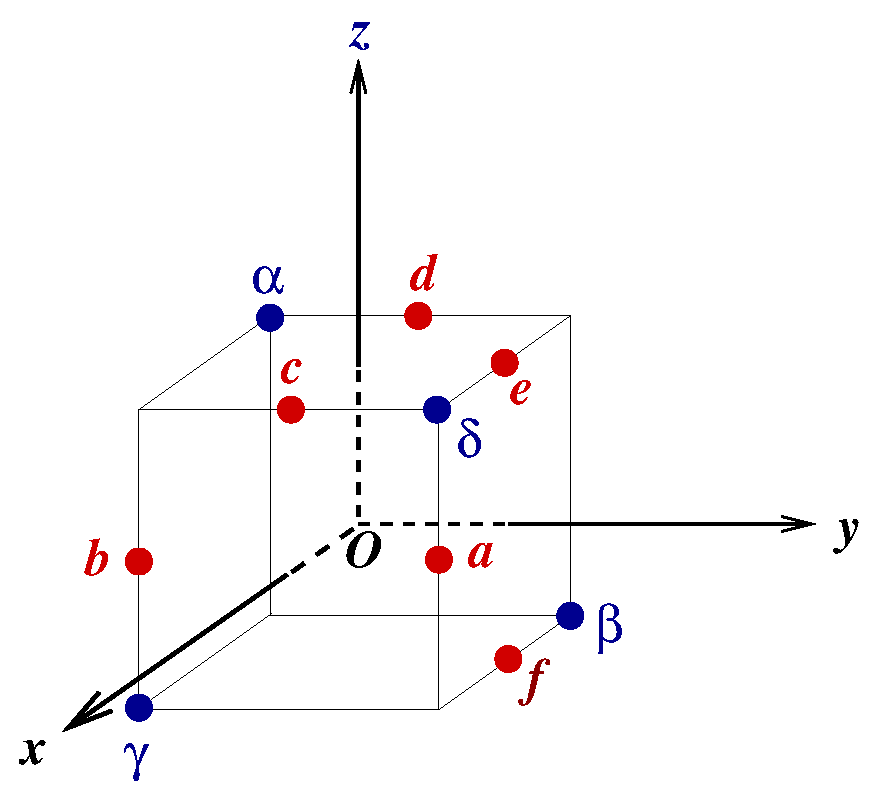
\includegraphics[scale=0.5]{figures/Oaxes.pdf}
        \caption{The rotation axes corresponding to the rotations $C_{nj}$. Figure taken from Ref.~\cite{}}
        \label{fig:rotation_axes}
    \end{figure}
    The octahedral point group, $O$, consists of all allowed rotations on a three-dimensional spatially-isotropic cubic lattice, and contains the following elements:
    \begin{table}[h!]
        \centering
        \begin{tabular}{l|l}
            Group element & Axes, $j$\\
            \hline
            $E$ & \\
            $C_{4j}$, $C_{4j}^{-1}$ & $x,y,z$ \\
            $C_{2j}$ & $x,y,z,a,b,c,d,e,f$ \\
            $C_{3j}$, $C_{3j}^{-1}$ & $\alpha,\beta,\gamma,\delta$
        \end{tabular}
        \label{table:O}
    \end{table}

    There are five irreps of $O$. Following the Mulliken convention~\cite{}, they are named $A_1$, $A_2$, $E$, $T_1$, $T_2$, and they have dimensions 1, 1, 2, 3, 3, respectively. In order to make connections to infinite-volume continuum physics, the Table~\ref{table:O_occurrence_nums} gives the \emph{occurrence numbers} $n_\Gamma^J$, which are the number of times the irrep $\Gamma$ of $O$ occurs in the subduction of the irrep $J$ of SO(3).

    When we take the direct product of $O$ with the group $\lbrace E,I_s \rbrace$, thereby adding in spatial inversions to our proper rotations, we get what is known as the point group $O_h$. This group has twice the number of irreps as $O$, and so we add the labels $g/u$ (standing for the German \emph{gerade} and \emph{ungerade}) to our irreps, which denote even and odd parity, respectively. The irreps of $O_h$ are $A_{1g}$, $A_{1u}$, $A_{2g}$, $A_{2u}$, $E_g$, $E_u$, $T_{1g}$, $T_{1u}$, $T_{2g}$, and $T_{2u}$.

    When we incorporate spin into the picture, we must introduce a new generator that represents rotating by $2\pi$ about any axis. Doing so, we arrive at the double octahedral point group $O^D$. Sparing the group-theoretical details, $O^D$ has three irreps in addition to all of the irreps of $O$. These are named $G_1$, $G_2$, and $H$, and are of dimension 2, 2, and 4, respectively. Table~\ref{table:OD_occurrence_nums} gives the occurrence numbers of these three additional numbers in the subductions of the $J$ irreps of SU(2). Like for $O_h$, when we incorporate spatial inversions into $O^D$, we arrive at the double point group $O_h^D$, which has twice the number of irreps of $O^D$. The additional irreps are $G_{1g}$, $G_{1u}$, $G_{2g}$, $G_{2u}$, $H_g$, and $H_u$.

    \renewcommand{\arraystretch}{1.2}
    \begin{table}
        \centering
        \begin{minipage}{.4\linewidth}
        \centering
        \begin{tabular}{l|l|l|l|l|l}
            $J$ & $n_{A_1}^J$ & $n_{A_2}^J$ & $n_{E}^J$ & $n_{T_1}^J$ & $n_{T_2}^J$\\
            \hline
            0 & 1 & 0 & 0 & 0 & 0\\
            1&0&0&0&1&0\\
            2&0&0&1&0&1\\
            3&0&1&0&1&1\\
            4&1&0&1&1&1\\
            \vdots & \vdots & \vdots & \vdots & \vdots & \vdots
        \end{tabular}
        \caption{}
        \label{table:O_occurrence_nums}
        \end{minipage}
        \begin{minipage}{.4\linewidth}
        \centering
        \begin{tabular}{l|l|l|l}
            $J$ & $n_{G_1}^J$ & $n_{G_2}^J$ & $n_{H}^J$ \\
            \hline
            $\frac{1}{2}$&1&0&0\\
            $\frac{3}{2}$&0&0&1\\
            $\frac{5}{2}$&0&1&1\\
            $\frac{7}{2}$&1&1&1\\
            $\frac{9}{2}$&1&0&2\\
            \vdots&\vdots&\vdots&\vdots
        \end{tabular}
        \caption{}
        \label{table:OD_occurrence_nums}
        \end{minipage}
    \end{table}
    \renewcommand{\arraystretch}{1.0}
    \subsubsection{Moving irreps}
    \subsection{Isospin and Quark Flavor}
    The physical mass of the up quark is $m_u = 2.16^{+0.49}_{-0.26}$ MeV and the physical mass of the down quark is $m_d = 4.67^{+0.48}_{-0.17}$ MeV~\cite{PhysRevD.98.030001}. While these masses differ by more than a factor of 2, their difference is very small compared to the next heaviest quark, which is the strange quark, measuring at $m_s = 93^{+11}_{-5}$ MeV~\cite{PhysRevD.98.030001}. Therefore, we find it justfied to make an approximation and set $m_u = m_d$ in our calculations. Since QCD conserves flavor (we do not include electroweak interactions), our theory now possesses an internal SU(2) symmetry, the conserved quantity of which is referred to as \emph{isospin}. This has the same mathematical structure as normal spin, and we can therefore think of it analogously, but it should be stressed that isospin has no relation to physical space and does not denote any kind of angular momentum. The up quark and down quark states can then be thought of as a doublet of states having total isospin $I=\frac{1}{2}$. Just like with SU(2) spin, isospin can be decomposed onto three axes. By convention, we assign the third isospin axis component of the up quark to be $I_3 = \frac{1}{2}$ and of the down quark to be $I_3 = -\frac{1}{2}$. Their corresponding antiparticles have the same $I$, but $I_3\rightarrow -I_3$. The work presented here is done in a theory of $N_f = 2 + 1$ QCD, meaning our theory contains two \emph{light} quarks, referring to the up and down quarks (the strange quark is sometimes referred to as a light quark in other contexts), and a strange quark.
    
    Under an SU(2) isospin rotation of the form
    \begin{equation}
        U_{R_{\tau}}=\exp (-i \varphi \cdot \tau),
    \end{equation}
    an operator $\overline O_{I_3}^{(I)}$ transforms according to the $I$ irreducible representation as
    
    

    \subsection{Charge Conjugation and $G$-Parity}

    \subsection{Projecting Operators onto Symmetry Sectors}

    \section{Single-Hadron Operator Construction}
    \subsubsection{Meson Operators}
    \subsubsection{Baryon Operators}
    \subsubsection{Tetraquark Operators}
    \section{Multi-Hadron Operator Construction}